\documentclass[12pt,a4paper]{article}
\usepackage[utf8]{inputenc}
\usepackage[T1]{fontenc}
\usepackage{amsmath, amssymb, amsfonts}
\usepackage{graphicx}
\usepackage{float}
\usepackage{geometry}
\usepackage{xcolor}
\usepackage{hyperref}
\geometry{margin=2.5cm}

\title{Newtonov zakon}
\author{Filip Jesenšek (28231064)}
\date{\today}

\begin{document}

\maketitle

\begin{abstract}
V poročilu obravnavamo numerično reševanje gibanja matematičnega nihala z različnimi metodami. Primerjamo Eulerjevo metodo, Heunovo metodo, Runge-Kutta metodo 4. reda, Verletovo metodo in PEFRL metodo. Pri tem se osredotočamo na njihovo natančnost, stabilnost in sposobnost ohranjanja energije sistema. Ugotovimo, da so simplektične metode, zlasti Verletova in PEFRL, daleč najboljše za dolgoročne simulacije, saj uspešno ohranjajo energijo in periodo nihanja tudi pri velikih korakih. V drugem delu poročila raziskujemo vsiljeno dušeno nihalo in van der Polov oscilator, kjer opazimo zanimive pojave, kot so bifurkacije, kaotično obnašanje in histereza.
\end{abstract}

\section{Uvod}

Gibanje masne točke v polju sil v eni dimenziji opisujemo z diferencialno enačbo drugega reda, znano kot Newtonov zakon. Ta zakon lahko zapišemo v obliki:

\begin{equation}
m \frac{d^2x}{dt^2} = F.
\end{equation}

Enačba je seveda enakovredna sistemu dveh enačb prvega reda, ki ga zapišemo kot:

\begin{equation}
m \frac{dx}{dt} = p, \quad \frac{dp}{dt} = F.
\end{equation}

V primeru matematičnega nihala je sila podana z izrazom $F = -mg\sin\theta$, kar vodi do diferencialne enačbe:

\begin{equation}
\frac{d^2\theta}{dt^2} = -\omega_0^2 \sin\theta,
\end{equation}

kjer je $\omega_0 = \sqrt{g/L}$ lastna krožna frekvenca nihala. Za majhne odmike lahko enačbo linearno aproksimiramo z $\sin\theta \approx \theta$ in dobimo harmonično nihanje, ki ga opisuje enačba:

\begin{equation}
\theta(t) = \theta_0 \sin(\omega_0 t + \phi_0).
\end{equation}

V splošnem primeru, ko odmiki niso majhni, pa se moramo za izračun nihajnega časa poslužiti specialnih funkcij. Natančen nihajni čas lahko izračunamo s pomočjo popolnega eliptičnega integrala prve vrste:

\begin{equation}
T_0 = \frac{4}{\omega_0} \int_0^{\pi/2} \frac{\mathrm{d}\varphi}{\sqrt{1 - \sin^2(\theta_0/2) \sin^2\varphi}} = \frac{4}{\omega_0} K(\sin^2(\theta_0/2)).
\end{equation}

Pri tem je $K(k)$ popolni eliptični integral prve vrste, $\theta_0$ pa amplituda nihanja. Za primer $\theta_0 = 1$ radian dobimo nihajni čas $T_0 \approx 6,74$ sekunde ob predpostavki $\omega_0 = 1$ rad/s.

\section{Numerične metode za reševanje diferencialnih enačb}

V nadaljevanju predstavljamo numerične metode, ki smo jih uporabili za reševanje enačbe matematičnega nihala. Vse metode smo implementirali s konstantnim korakom integracije $h$. Pri tem smo izhajali iz zapisa sistema diferencialnih enačb v obliki $\dot{\mathbf{y}} = \mathbf{f}(\mathbf{y})$, kjer je $\mathbf{y} = (\theta, \dot{\theta})^T$.

\subsection{Eulerjeva metoda}

Eulerjeva metoda je najpreprostejša numerična metoda za reševanje diferencialnih enačb. Napredujemo s konstantnim korakom $h$ po predpisu:

\begin{equation}
\mathbf{y}_{n+1} = \mathbf{y}_n + h \mathbf{f}(\mathbf{y}_n).
\end{equation}

Metoda je eksplicitna in ima lokalno napako reda $O(h^2)$, globalno napako pa reda $O(h)$. To pomeni, da je metoda razmeroma netočna in zahteva zelo majhne korake za zadovoljivo natančnost. Poleg tega je Eulerjeva metoda pogosto numerično nestabilna, zlasti pri večjih korakih.

\subsection{Heunova metoda}

Heunova metoda spada v družino metod tipa prediktor-korektor. Najprej izračunamo prediktor po Eulerjevi metodi, nato pa popravimo vrednost s povprečjem dveh odvodov. Algoritem lahko zapišemo kot:

\begin{align}
\mathbf{k}_1 &= \mathbf{f}(\mathbf{y}_n), \\
\mathbf{k}_2 &= \mathbf{f}(\mathbf{y}_n + h \mathbf{k}_1), \\
\mathbf{y}_{n+1} &= \mathbf{y}_n + \frac{h}{2}(\mathbf{k}_1 + \mathbf{k}_2).
\end{align}

Heunova metoda ima globalno napako reda $O(h^2)$, kar pomeni, da je za red velikosti natančnejša od Eulerjeve metode. Je tudi bolj stabilna od Eulerjeve metode, vendar še vedno ne ohranja energije sistema pri dolgoročnih simulacijah.

\subsection{Runge-Kutta metoda 4. reda}

Runge-Kutta metoda 4. reda (RK4) je ena najbolj razširjenih metod za reševanje diferencialnih enačb. Za izračun naslednjega koraka potrebujemo štiri ocene odvoda na intervalu $[t_n, t_{n+1}]$:

\begin{align}
\mathbf{k}_1 &= \mathbf{f}(\mathbf{y}_n), \\
\mathbf{k}_2 &= \mathbf{f}(\mathbf{y}_n + \tfrac{h}{2}\mathbf{k}_1), \\
\mathbf{k}_3 &= \mathbf{f}(\mathbf{y}_n + \tfrac{h}{2}\mathbf{k}_2), \\
\mathbf{k}_4 &= \mathbf{f}(\mathbf{y}_n + h \mathbf{k}_3), \\
\mathbf{y}_{n+1} &= \mathbf{y}_n + \tfrac{h}{6}(\mathbf{k}_1 + 2\mathbf{k}_2 + 2\mathbf{k}_3 + \mathbf{k}_4).
\end{align}

RK4 metoda ima globalno napako reda $O(h^4)$, kar pomeni, da je izjemno natančna že pri zmerno majhnih korakih. Je tudi zelo stabilna in se uporablja kot standardna metoda v mnogih programskih knjižnicah. Vendar tudi RK4 metoda ni simplektična, kar pomeni, da pri dolgoročnih simulacijah ne ohranja energije sistema.

\subsection{Verletova metoda}

Verletova metoda (znana tudi kot Störmerjeva metoda) je simplektična metoda drugega reda. Simplektične metode so posebej primerne za reševanje Hamiltonovih sistemov, saj približno ohranjajo energijo sistema tudi pri dolgoročnih simulacijah. Verletovo metodo lahko zapišemo v več enakovrednih oblikah. Ena izmed njih je:

\begin{align}
\theta_{n+1} &= \theta_n + h \dot{\theta}_n + \frac{h^2}{2} f(\theta_n), \\
\dot{\theta}_{n+1} &= \dot{\theta}_n + \frac{h}{2} [f(\theta_n) + f(\theta_{n+1})].
\end{align}

Pri tem je $f(\theta) = -\omega_0^2 \sin\theta$ pospešek nihala. Verletovo metodo lahko zapišemo tudi v obliki središčnih diferenc, kjer nas hitrost ne zanima neposredno:

\begin{equation}
\theta_{n+1} - 2\theta_n + \theta_{n-1} = h^2 f(\theta_n).
\end{equation}

Alternativno lahko shemo zapišemo s pomočjo vmesnih točk, kjer preskakujemo med lego in hitrostjo z zamikom $h/2$. Ta zapis je znan pod angleškim imenom \textit{leapfrog}:

\begin{align}
\theta_{n+1} &= \theta_n + h \dot{\theta}_{n+1/2}, \\
\dot{\theta}_{n+3/2} &= \dot{\theta}_{n+1/2} + h f(\theta_{n+1}).
\end{align}

Verletova metoda je globalno natančna do drugega reda in točno ohranja vrtilno količino sistema, kadar je ta smiselna. Kljub nižjemu redu natančnosti v primerjavi z RK4 metodo je zaradi simplektičnosti pogosto boljša izbira za dolgoročne simulacije dinamičnih sistemov.

\subsection{PEFRL metoda}

PEFRL (Position Extended Forest-Ruth Like) metoda je simplektična metoda četrtega reda, ki predstavlja izboljšavo osnovne Forest-Ruthove metode. Je ena najbolj natančnih simplektičnih metod, primerna za zelo dolge simulacije. Metoda uporablja naslednje koeficiente, ki so bili optimizirani za minimalno napako: $\xi = 0,1786178958448091$, $\lambda = -0,2123418310626054$ in $\chi = -0,06626458266981843$. Algoritem PEFRL metode lahko zapišemo kot zaporedje korakov:

\begin{align}
p &\leftarrow p + \xi h f(q), \\
q &\leftarrow q + \lambda h p, \\
p &\leftarrow p + \chi h f(q), \\
q &\leftarrow q + (1-2\lambda) h p, \\
p &\leftarrow p + \chi h f(q), \\
q &\leftarrow q + \lambda h p, \\
p &\leftarrow p + \xi h f(q).
\end{align}

Ti koeficienti so rezultat reševanja kompleksnega sistema nelinearnih enačb, ki zagotavljajo, da je metoda četrtega reda in simplektična. PEFRL metoda je zato izjemno natančna in primerna za najzahtevnejše simulacije, kjer je potrebno ohranjanje energije na dolgih časovnih skalah.

\section{Metodologija testiranja}

\subsection{Merjenje nihajnega časa}

Nihajni čas smo definirali kot čas med dvema zaporednima maksimumoma odmika nihala. Začetna točka je po definiciji maksimum, saj nihalo začnemo iz mirovanja pri maksimalnem odmiku. Za iskanje ostalih maksimumov smo uporabili funkcijo \texttt{find\_peaks} iz knjižnice \texttt{scipy.signal}.

Vendar pa bi uporaba preprostega iskanja maksimumov omejila natančnost na velikost koraka integracije $h$. Za želeno natančnost treh decimalnih mest bi tako potrebovali izjemno majhen korak velikosti $10^{-3}$ s, kar je računsko zelo potratno. Zato smo uporabili izboljšano metodo: okoli vsakega maksimuma smo graf aproksimirali s kvadratno funkcijo, podano s tremi točkami okoli maksimuma. Naj bodo to točke $(x_1, y_1)$, $(x_2, y_2)$ in $(x_3, y_3)$, pri čemer je $x_2$ točka najbližja maksimumu. Koeficiente lokalnega kvadratnega približka $f(x) \approx ax^2 + bx + c$ smo izračunali po formulah:

\begin{equation}
a = \frac{(y_1-y_2)(x_1-x_3) - (y_1-y_3)(x_1-x_2)}{(x_1-x_2)(x_1-x_3)(x_2-x_3)},
\end{equation}

\begin{equation}
b = \frac{y_1-y_2}{x_1-x_2} - a(x_1+x_2),
\end{equation}

\begin{equation}
c = y_1 - ax_1^2 - bx_1.
\end{equation}

Maksimum kvadratnega približka je nato v točki:

\begin{equation}
x_{\text{max}} = -\frac{b}{2a}, \qquad f_{\text{max}} = c - \frac{b^2}{4a}.
\end{equation}

Ta postopek kvadratne interpolacije nam je omogočil bistveno natančnejšo določitev nihajnega časa, saj smo s tremi točkami lahko zelo natančno določili položaj maksimuma, ne glede na velikost koraka.

\subsection{Spremljanje energije}

Pri matematičnem nihalu je skupna mehanska energija podana z vsoto kinetične in potencialne energije. V normaliziranih enotah, kjer je masa $m=1$ in $gL=1$, lahko energijo zapišemo kot:

\begin{equation}
E = \frac{1}{2} \dot{\theta}^2 + \omega_0^2 (1 - \cos\theta).
\end{equation}

Začetna energija pri odmiku $\theta_0 = 1$ radian in začetni hitrosti $\dot{\theta}=0$ znaša $E_0 = 1 - \cos(1) \approx 0,4597$. Pri numeričnih simulacijah smo spremljali relativno napako energije, definirano kot:

\begin{equation}
\Delta E_{\text{rel}}(t) = \frac{E(t) - E_0}{E_0} \cdot 100\%.
\end{equation}

Ta količina nam pove, koliko se numerična rešitev oddalji od prave energije sistema. Pri idealnih metodah bi morala biti napaka energije ves čas enaka nič, vendar so vse numerične metode le približne in zato s časom uvajajo napake.

\subsection{Testiranje stabilnosti periode}

Za testiranje dolgoročne stabilnosti posamezne metode smo simulirali nihanje čez 20 nihajev s korakom $\Delta t = 0,1$ s. Za vsak zaporedni nihaj smo izračunali nihajni čas in ga primerjali z analitično vrednostjo. Tako smo lahko opazovali, kako se napaka periode spreminja s časom. Pri stabilnih metodah pričakujemo, da napaka periode ostaja približno konstantna, medtem ko pri nestabilnih metodah napaka linearno narašča s časom.

\section{Rezultati in analiza}

\subsection{Primerjava natančnosti metod}

Slika \ref{fig:error_analysis} prikazuje odvisnost maksimalne napake od velikosti koraka za vseh pet testiranih metod. Graf prikazuje maksimalno napako pri simulaciji do časa 15 sekund.

\begin{figure}[H]
    \centering
    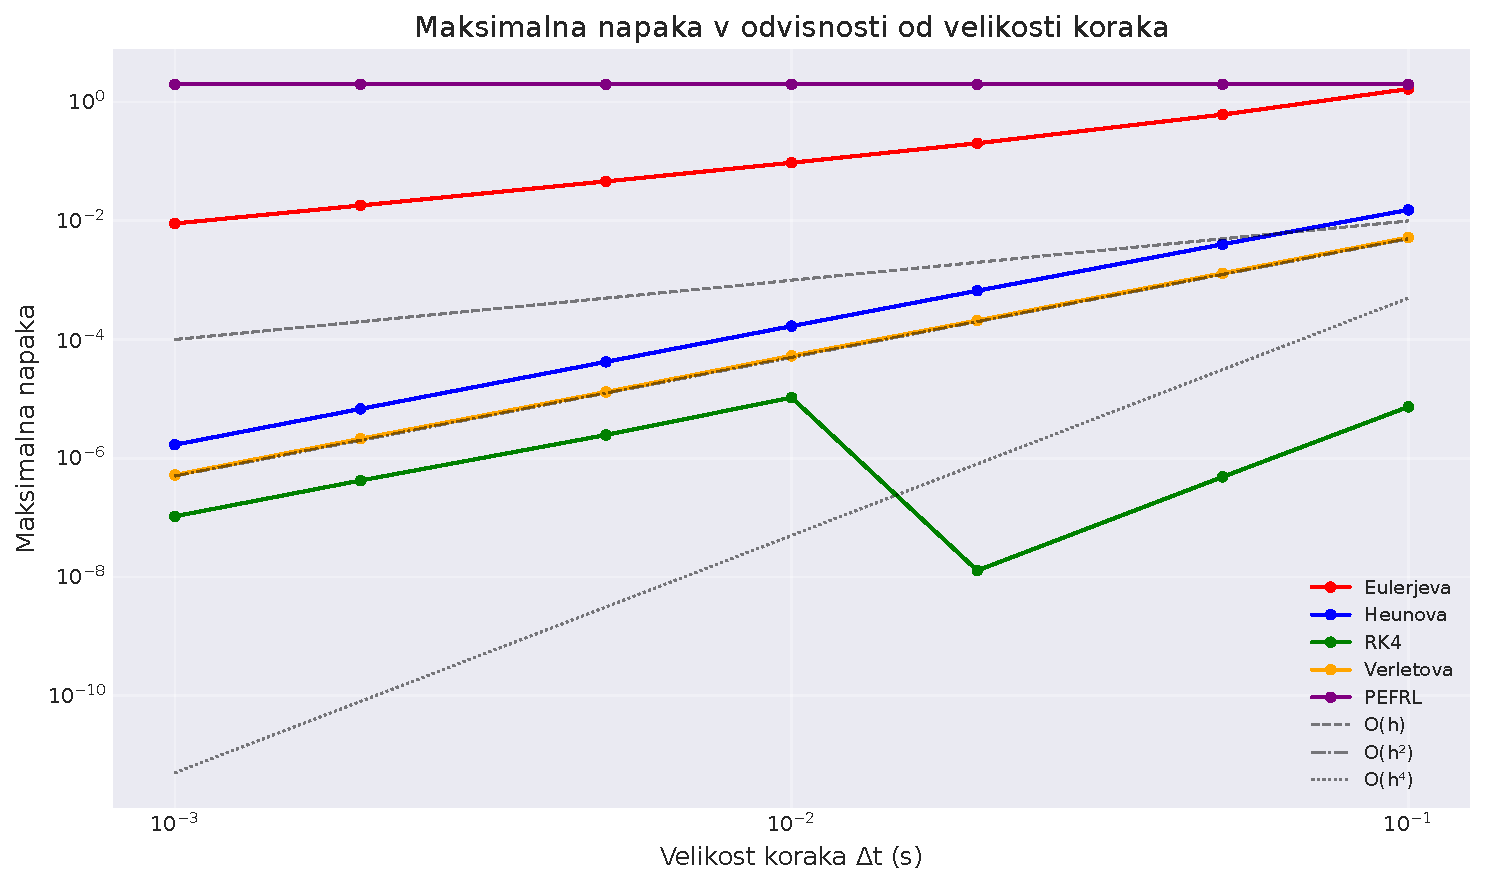
\includegraphics[width=0.9\textwidth]{slika4_analiza_napak.pdf}
    \caption{Maksimalna napaka v odvisnosti od velikosti koraka. S črnimi črtami so označene asimptotske odvisnosti $O(h)$, $O(h^2)$ in $O(h^4)$.}
    \label{fig:error_analysis}
\end{figure}

Iz slike je razvidno, da Eulerjeva metoda doseže le linearno konvergenco, kar se kaže v naklonu premice približno 1 na log-log grafu. Heunova in Verletova metoda (oba drugega reda) dosežeta kvadratno konvergenco z naklonom 2, medtem ko RK4 in PEFRL (oba četrtega reda) dosežeta konvergenco četrtega reda z naklonom 4. To je v popolnem skladu s teoretičnimi pričakovanji. Zanimivo je, da se simplektični metodi (Verlet in PEFRL) pri enaki globalni natančnosti izkažeta za nekoliko boljši od nesimplektičnih ekvivalentov, kar je posebej opazno pri primerjavi Verletove in Heunove metode.

Tabela \ref{tab:step_sizes} prikazuje potrebne velikosti koraka za dosego natančnosti treh decimalnih mest pri določitvi periode. Vidimo lahko, da Eulerjeva metoda zahteva izjemno majhen korak $5,3 \cdot 10^{-4}$ s, kar je posledica njene nizke natančnosti. Heunova in Verletova metoda potrebujeta korak velikosti nekaj stotink sekunde, medtem ko RK4 in PEFRL zmoreta enako natančnost doseči že s korakom velikosti približno pol sekunde. PEFRL metoda se pri tem izkaže za najboljšo, saj zadošča že korak $\Delta t = 0,57$ s, kar je skoraj 1000-krat večji korak kot pri Eulerjevi metodi.

\begin{table}[H]
\centering
\caption{Potrebna velikost koraka za natančnost treh decimalnih mest}
\label{tab:step_sizes}
\begin{tabular}{|c|c|}
\hline
\textbf{Metoda} & \textbf{Korak $\Delta t$ [s]} \\
\hline
Eulerjeva & $5,3 \cdot 10^{-4}$ \\
Heunova & $3,6 \cdot 10^{-2}$ \\
RK4 & $0,40$ \\
Verletova & $6,3 \cdot 10^{-2}$ \\
PEFRL & $0,57$ \\
\hline
\end{tabular}
\end{table}

\subsection{Dolgoročna stabilnost in ohranjanje energije}

Slika \ref{fig:stability} prikazuje dolgoročno obnašanje metod s fiksnim korakom $\Delta t = 0,1$ s. Na levem grafikonu (a) vidimo relativno napako energije v odvisnosti od časa, na srednjem grafikonu (b) pa napako periode skozi več zaporednih nihajev. Desni grafikon (c) prikazuje povečavo energije pri simplektičnih metodah, kjer so napake veliko manjše.

\begin{figure}[H]
    \centering
    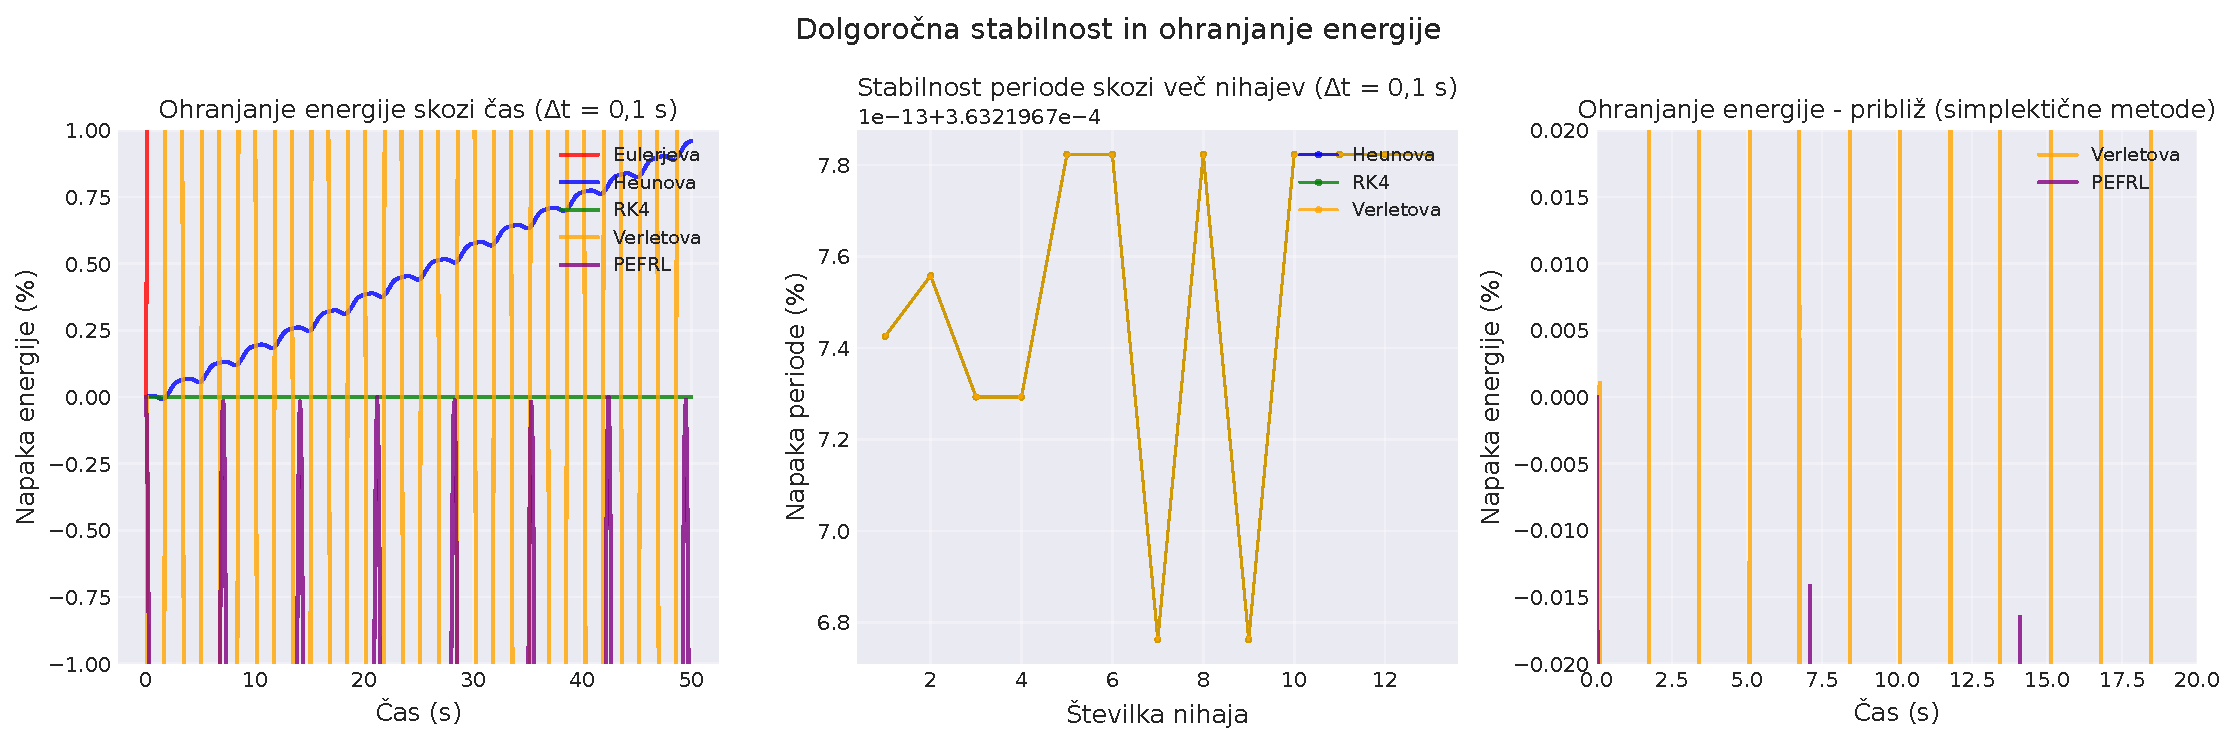
\includegraphics[width=0.9\textwidth]{slika5_stabilnost.pdf}
    \caption{Dolgoročna stabilnost in ohranjanje energije. Levo (a): Relativna napaka energije v odvisnosti od časa. Sredina (b): Relativna napaka periode skozi več zaporednih nihajev. Desno (c): Povečava napake energije pri Verletovi in PEFRL metodi.}
    \label{fig:stability}
\end{figure}

Pri nesimplektičnih metodah (Eulerjeva, Heunova in RK4) opazimo, da se napaka energije s časom linearno oddaljuje od ničle. Pri Eulerjevi metodi napaka že po nekaj sekundah preseže 100\%, kar pomeni, da metoda popolnoma odpove. Heunova metoda je nekoliko boljša, vendar tudi pri njej napaka energije narašča približno linearno in po 50 sekundah doseže približno 0,5\%. RK4 metoda se obnese presenetljivo dobro, saj je napaka energije po 50 sekundah le približno $10^{-4}\%$, kar je izjemno dober rezultat. Vendar tudi pri RK4 metodi napaka narašča s časom, čeprav zelo počasi.

Pri simplektičnih metodah (Verlet in PEFRL) je situacija povsem drugačna. Napaka energije ne narašča linearno s časom, ampak ostaja omejena in niha okoli neke konstantne vrednosti. Pri Verletovi metodi napaka energije niha z amplitudo približno $10^{-2}\%$, medtem ko je pri PEFRL metodi ta amplituda približno $10^{-4}\%$. Še pomembneje pa je, da se napaka ne povečuje s časom, kar pomeni, da simplektične metode ohranjajo energijsko skalirano orbito tudi pri zelo dolgih simulacijah. Ta lastnost je izjemno pomembna pri simulacijah planetarnih sistemov ali drugih dolgotrajnih dinamičnih pojavov.

Podobno sliko vidimo pri napaki periode na srednjem grafikonu. Pri nesimplektičnih metodah napaka periode linearno narašča s številom nihajev, kar pomeni, da se nihalo postopoma desinhronizira. Pri simplektičnih metodah pa napaka periode ostaja konstantna, kar pomeni, da nihalo ohranja pravilen takt tudi po mnogih nihajih.

\subsection{Fazni portreti}

Slika \ref{fig:phase_portraits} prikazuje fazne portrete matematičnega nihala za različne začetne pogoje. Fazni prostor je dvodimenzionalen, pri čemer sta koordinati odmik $\theta$ in hitrost $\dot{\theta}$. Barva poti označuje čas, pri čemer temno modra ustreza začetku, rumena pa koncu simulacije.

\begin{figure}[H]
    \centering
    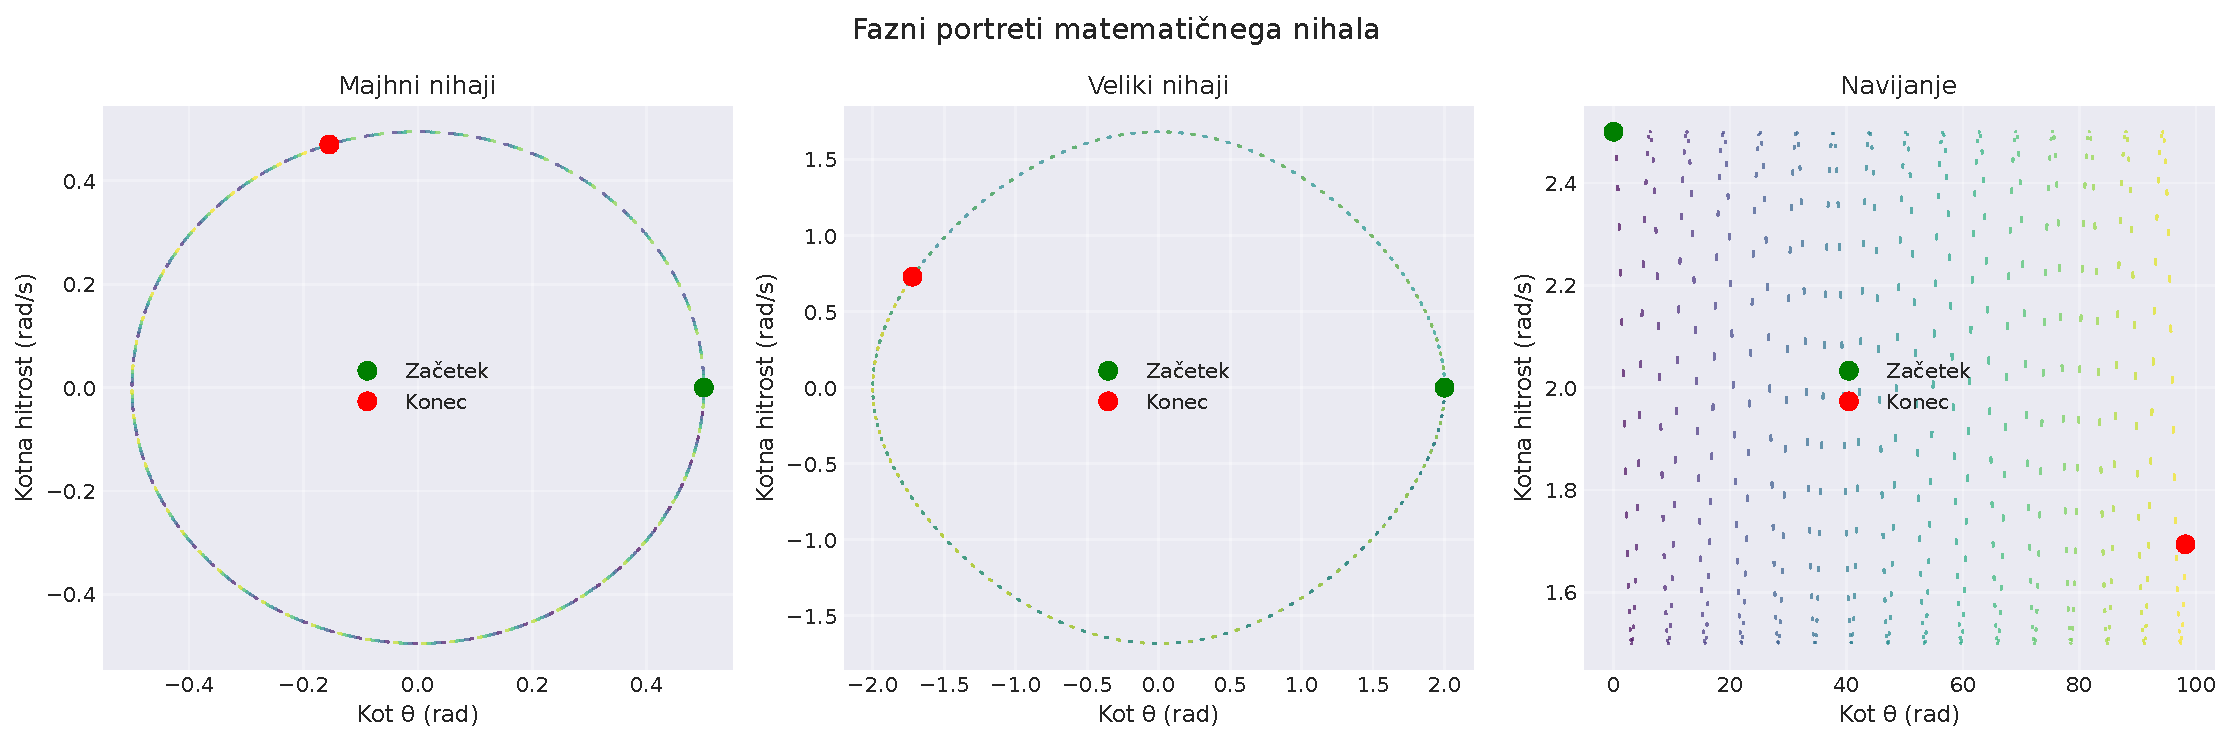
\includegraphics[width=0.9\textwidth]{slika2_fazni_portreti.pdf}
    \caption{Fazni portreti matematičnega nihala. Levo: majhni nihaji ($\theta_0 = 0,5$ rad). Sredina: veliki nihaji ($\theta_0 = 2,0$ rad). Desno: navijanje ($\dot{\theta}_0 = 2,5$ rad/s).}
    \label{fig:phase_portraits}
\end{figure}

Na levem grafikonu vidimo primer majhnih nihajev z začetnim odmikom $\theta_0 = 0,5$ radiana. Fazni portret je skoraj popolna krožnica, kar ustreza harmoničnemu oscilatorju. To je pričakovano, saj je pri majhnih odmikih $\sin\theta \approx \theta$ in sistem postane linearen. Na srednjem grafikonu so prikazani veliki nihaji z začetnim odmikom $\theta_0 = 2,0$ radiana. Fazni portret se raztegne v podolgovato obliko, ki spominja na oko. To je posledica nelinearnosti, saj pri velikih odmikih nihalo dlje časa preživi v skrajnih legah, kjer je hitrost majhna. Desni grafikon prikazuje primer navijanja, kjer začetna hitrost $\dot{\theta}_0 = 2,5$ rad/s zadostuje, da nihalo premaga potencialno oviro in začne krožiti okoli osi. V tem primeru fazni portret ni več sklenjena krivulja, ampak se nihalo premika vedno bolj v desno in vsak obrat ustreza spremembi odmika za $2\pi$.

\subsection{Vsiljeno dušeno nihalo}

V drugem delu naloge smo raziskovali vsiljeno dušeno matematično nihalo, ki ga opisuje naslednja diferencialna enačba:

\begin{equation}
\frac{d^2\theta}{dt^2} + \beta \frac{d\theta}{dt} + \sin\theta = v \cos(\omega t).
\end{equation}

Pri tem je $\beta$ koeficient dušenja, $v$ amplituda vzbujevalne sile, $\omega$ pa njena krožna frekvenca. Sistem ima tri prostostne stopnje ($\theta$, $\dot{\theta}$ in fazo vzbujanja $\omega t$), zato lahko pričakujemo pojav kaosa. Slika \ref{fig:driven_regimes} prikazuje osem različnih dinamičnih režimov, ki se pojavijo pri koeficientu dušenja $\beta = 0,5$ in različnih parametrih vzbujanja.

\begin{figure}[H]
    \centering
    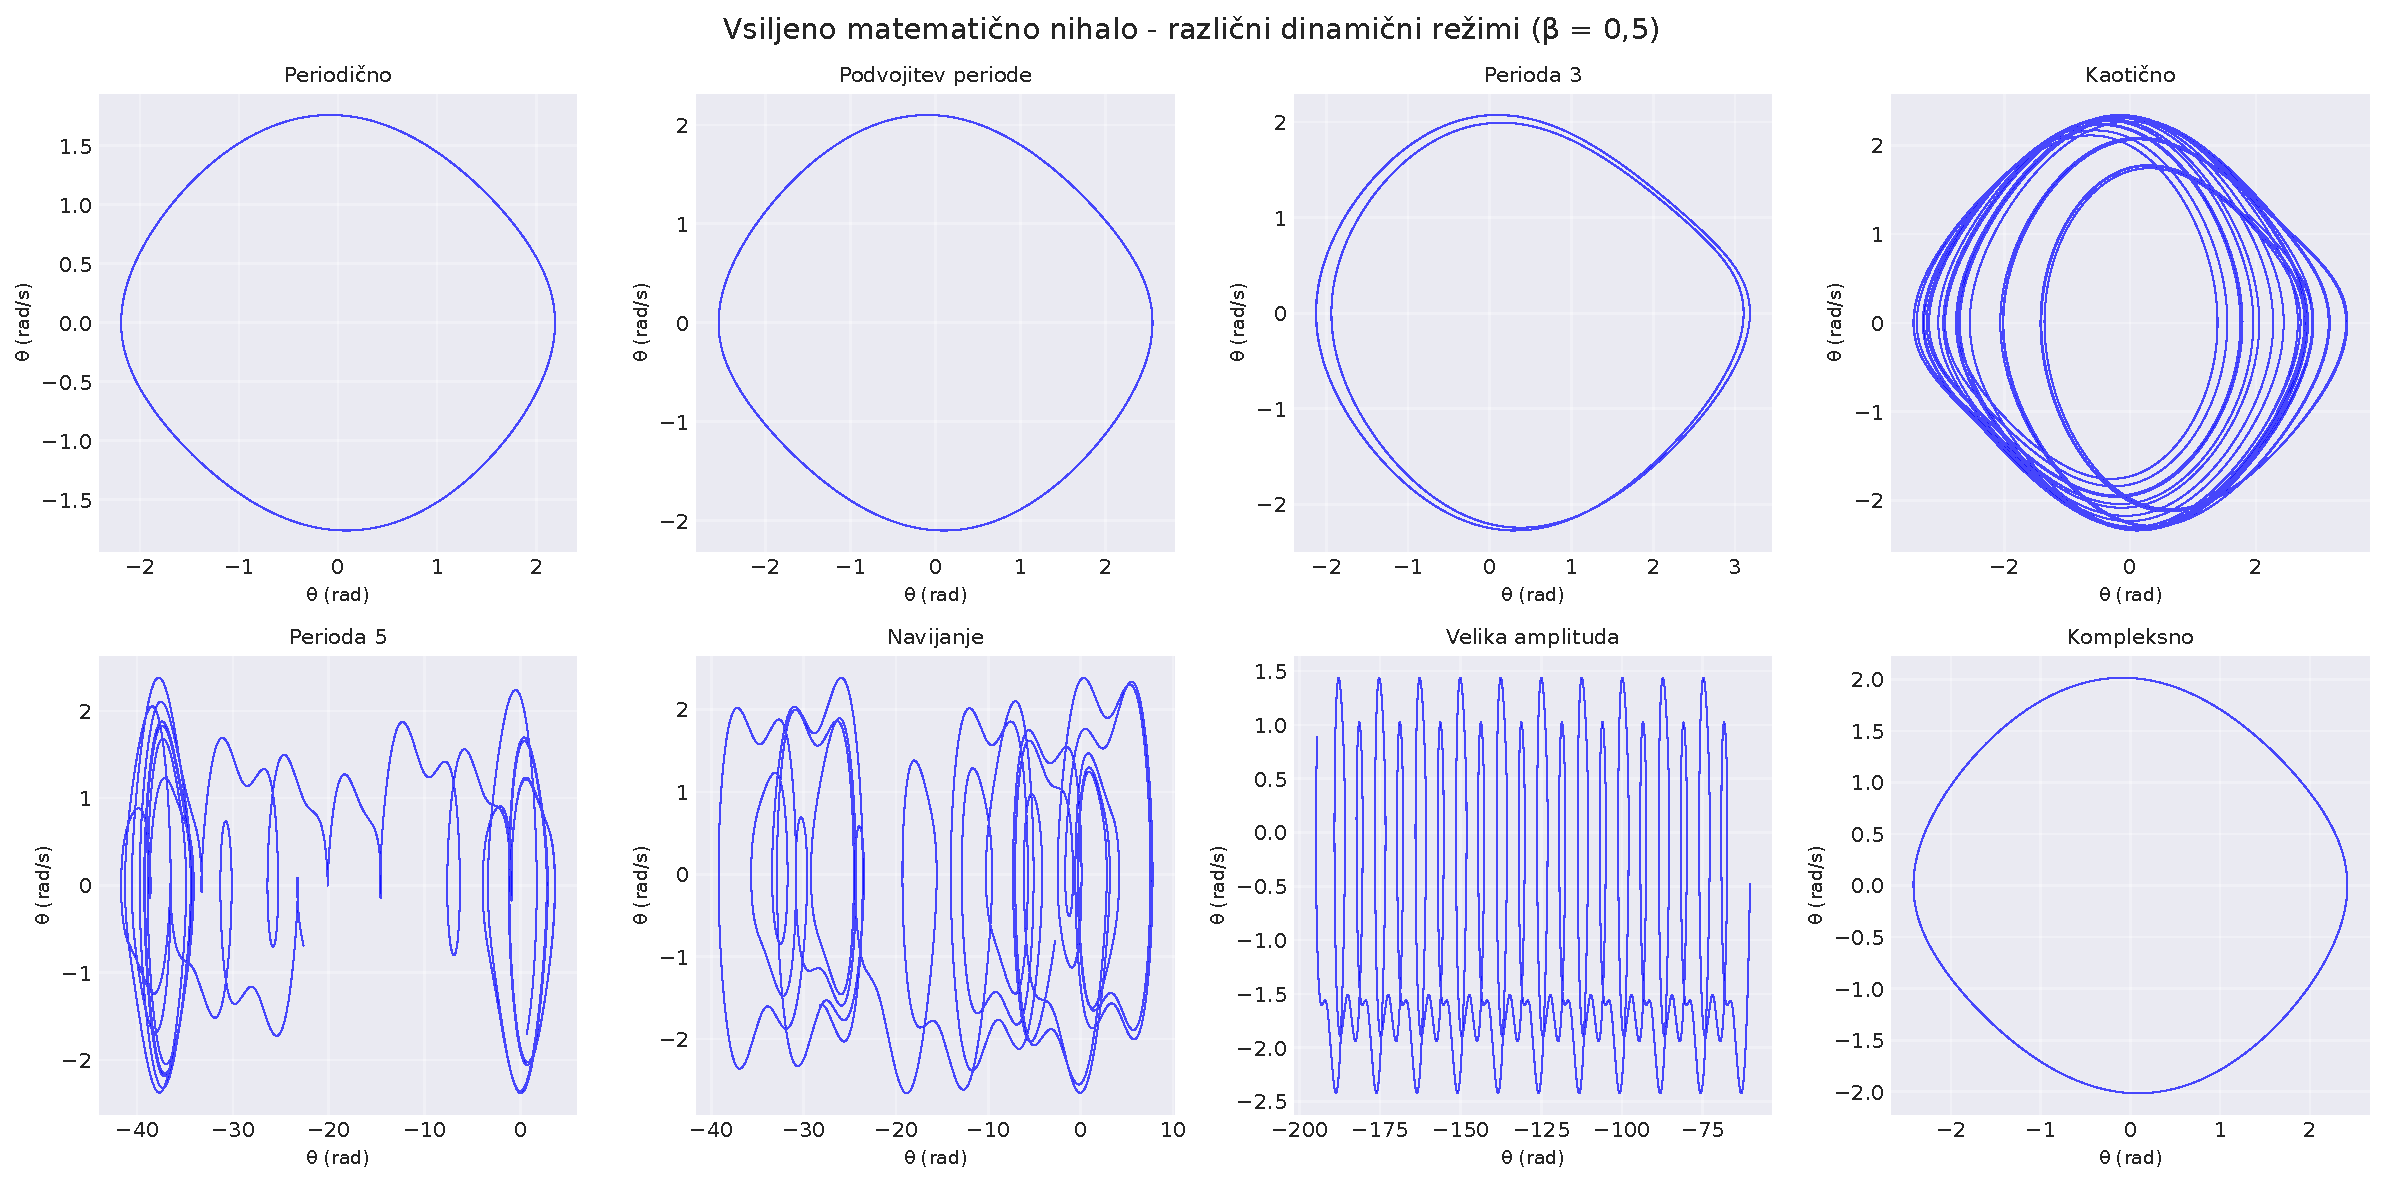
\includegraphics[width=0.9\textwidth]{slika9_vsiljeno_nihalo_rezimi.pdf}
    \caption{Različni dinamični režimi vsiljenega matematičnega nihala pri $\beta = 0,5$. Od leve proti desni in od zgoraj navzdol: periodično nihanje, podvojitev periode, perioda 3, kaotično nihanje, perioda 5, navijanje, nihanje z veliko amplitudo in kompleksno nihanje.}
    \label{fig:driven_regimes}
\end{figure}

Pri majhnih amplitudah vzbujanja (prvi grafikon zgoraj levo) opazimo periodično nihanje, kjer se sistem odziva z enako periodo kot vzbujevalna sila. Ko povečamo amplitudo vzbujanja, lahko opazimo bifurkacijo s podvojitvijo periode (prvi grafikon zgoraj desno), kjer je vsaka druga amplituda nekoliko manjša. Pri nadaljnjem povečevanju amplitude lahko pride do prehoda v kaotično obnašanje (drugi grafikon zgoraj desno), kjer je pot nihala popolnoma nepredvidljiva, čeprav je sistem povsem determinističen. Posebej zanimiv je primer navijanja (drugi grafikon spodaj levo), kjer nihalo zaradi dovolj močne vzbujevalne sile začne krožiti okoli osi in se stalno vrti v eno smer. V nekaterih primerih opazimo tudi nihanje okoli nestabilne ravnovesne lege pri $\theta = \pi$ (obrnjeno nihalo), kar je možno le s pravilno izbiro parametrov vzbujanja.

\subsection{Resonančne krivulje}

Slika \ref{fig:resonance} prikazuje resonančne krivulje za različne amplitude vzbujanja. Resonančna krivulja prikazuje odvisnost amplitude odziva sistema od frekvence vzbujanja.

\begin{figure}[H]
    \centering
    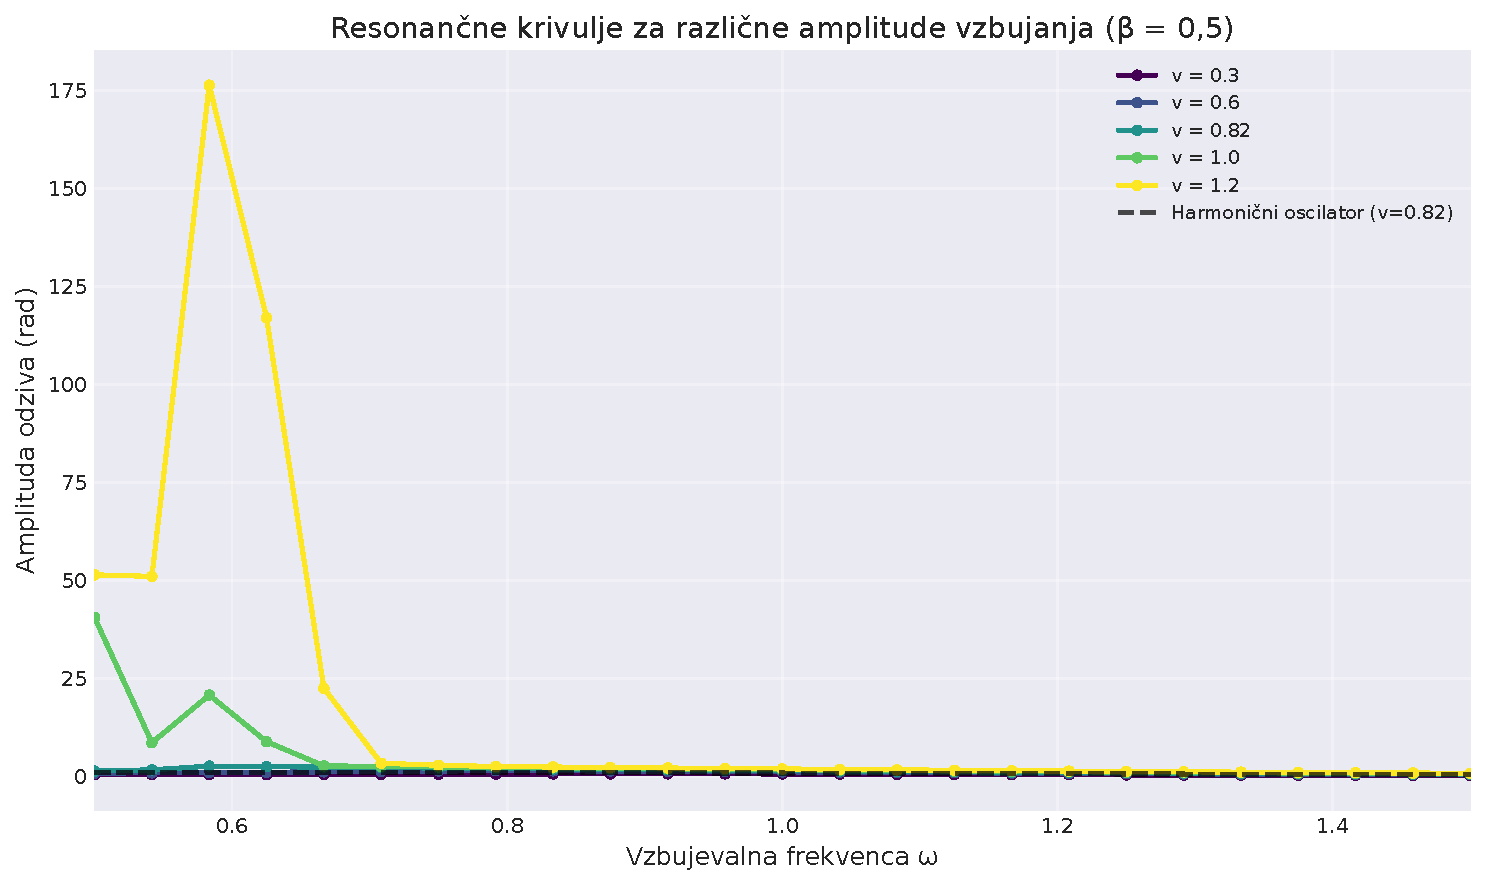
\includegraphics[width=0.9\textwidth]{slika12_resonancne_krivulje.pdf}
    \caption{Resonančne krivulje za različne amplitude vzbujanja pri $\beta = 0,5$. Črtkana črta prikazuje harmonični oscilator za primerjavo.}
    \label{fig:resonance}
\end{figure}

Pri majhnih amplitudah vzbujanja (na primer $v = 0,3$) je resonančna krivulja podobna tisti pri harmoničnem oscilatorju, z vrhom pri lastni frekvenci $\omega = 1$. Ko povečujemo amplitudo vzbujanja, se vrh resonančne krivulje začne pomikati proti nižjim frekvencam, kar je značilno za nelinearne sisteme z mehčajočo karakteristiko. Pri $v = 0,82$ opazimo, da krivulja postane zelo strma, kar nakazuje na pojav histereze.

\subsection{Histereza}

Slika \ref{fig:hysteresis} prikazuje histerezni pojav v sistemu pri nizkem dušenju $\beta = 0,03$ in majhni amplitudi vzbujanja $v = 0,03$. V tem primeru je sistem zelo blizu Duffingovemu oscilatorju, kjer je histereza dobro poznan pojav.

\begin{figure}[H]
    \centering
    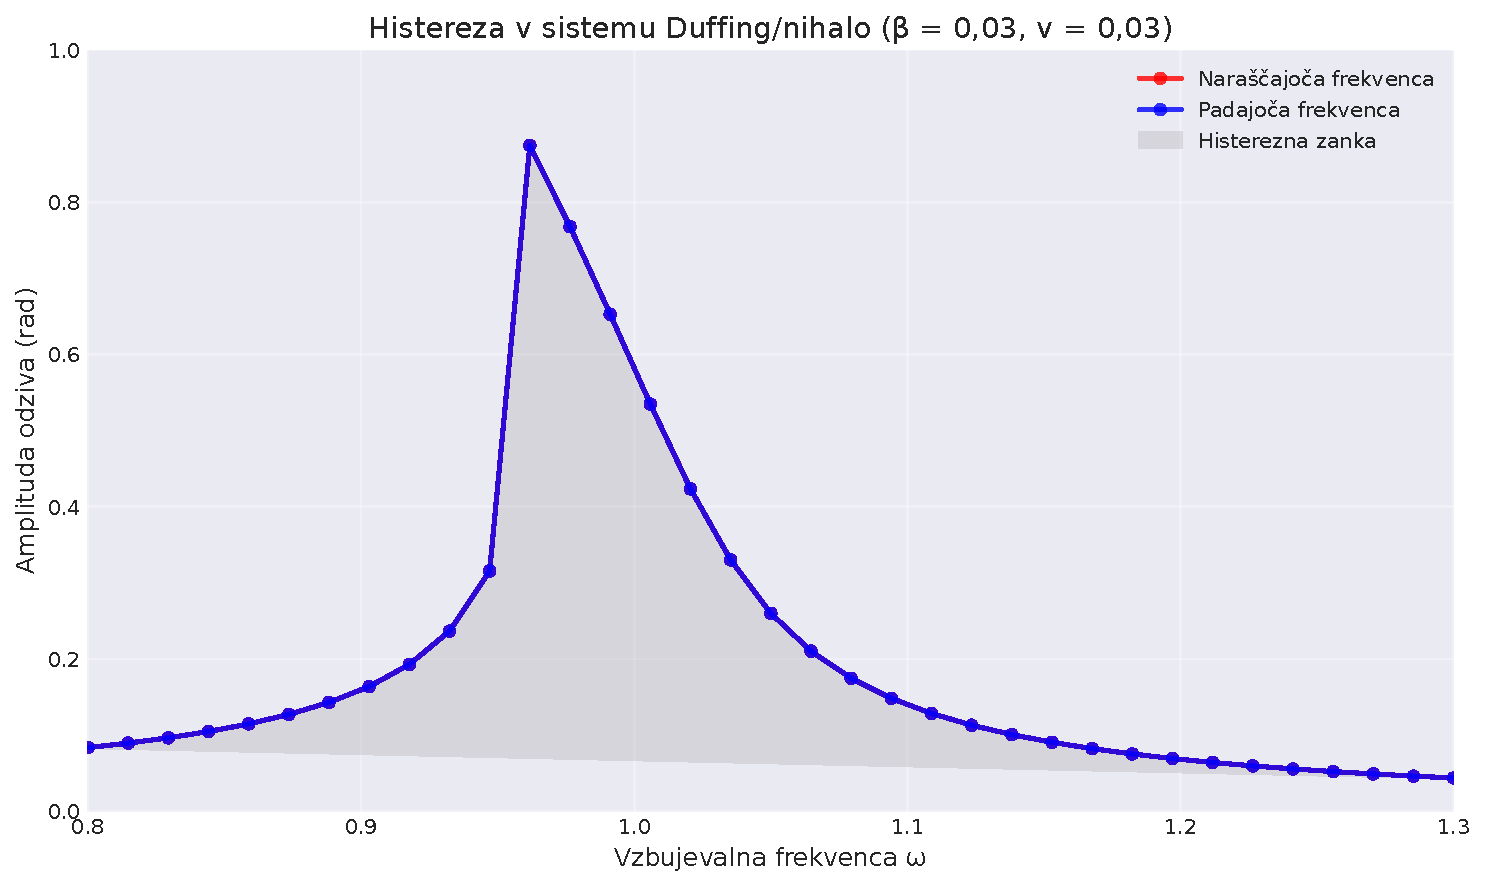
\includegraphics[width=0.9\textwidth]{slika13_histereza.pdf}
    \caption{Histereza v sistemu Duffing/nihalo pri $\beta = 0,03$ in $v = 0,03$. Rdeča krivulja prikazuje odziv pri naraščajoči frekvenci, modra pa pri padajoči frekvenci. Osenčeno območje predstavlja histerezno zanko.}
    \label{fig:hysteresis}
\end{figure}

Pri histerezi ima sistem pri isti frekvenci vzbujanja lahko dva različna stabilna odziva, odvisno od zgodovine sistema. Če frekvenco vzbujanja počasi povečujemo, sistem sledi zgornji veji krivulje (rdeča črta), če pa frekvenco počasi zmanjšujemo, sledi spodnji veji (modra črta). Osenčeno območje med obema krivuljama predstavlja histerezno zanko. Ta pojav je značilen za nelinearne sisteme in ga v linearnih sistemih ne moremo opaziti.

\subsection{Van der Polov oscilator}

Van der Polov oscilator je nelinearni sistem, ki ga opisuje naslednja diferencialna enačba:

\begin{equation}
\frac{d^2x}{dt^2} - \lambda (1-x^2)\frac{dx}{dt} + x = v \cos(\omega t).
\end{equation}

Pri $\lambda > 0$ ima nihanje lastnost, da se za majhne odmike dušenje obnaša negativno (sistem črpa energijo), za velike odmike pa pozitivno (sistem izgublja energijo). Posledica tega je obstoj stabilnega limitnega cikla. Slika \ref{fig:vanderpol} prikazuje fazne portrete van der Polovega oscilatorja za različne vrednosti parametra $\lambda$ pri fiksnih parametrih vzbujanja $v = 10$ in $\omega = 1$.

\begin{figure}[H]
    \centering
    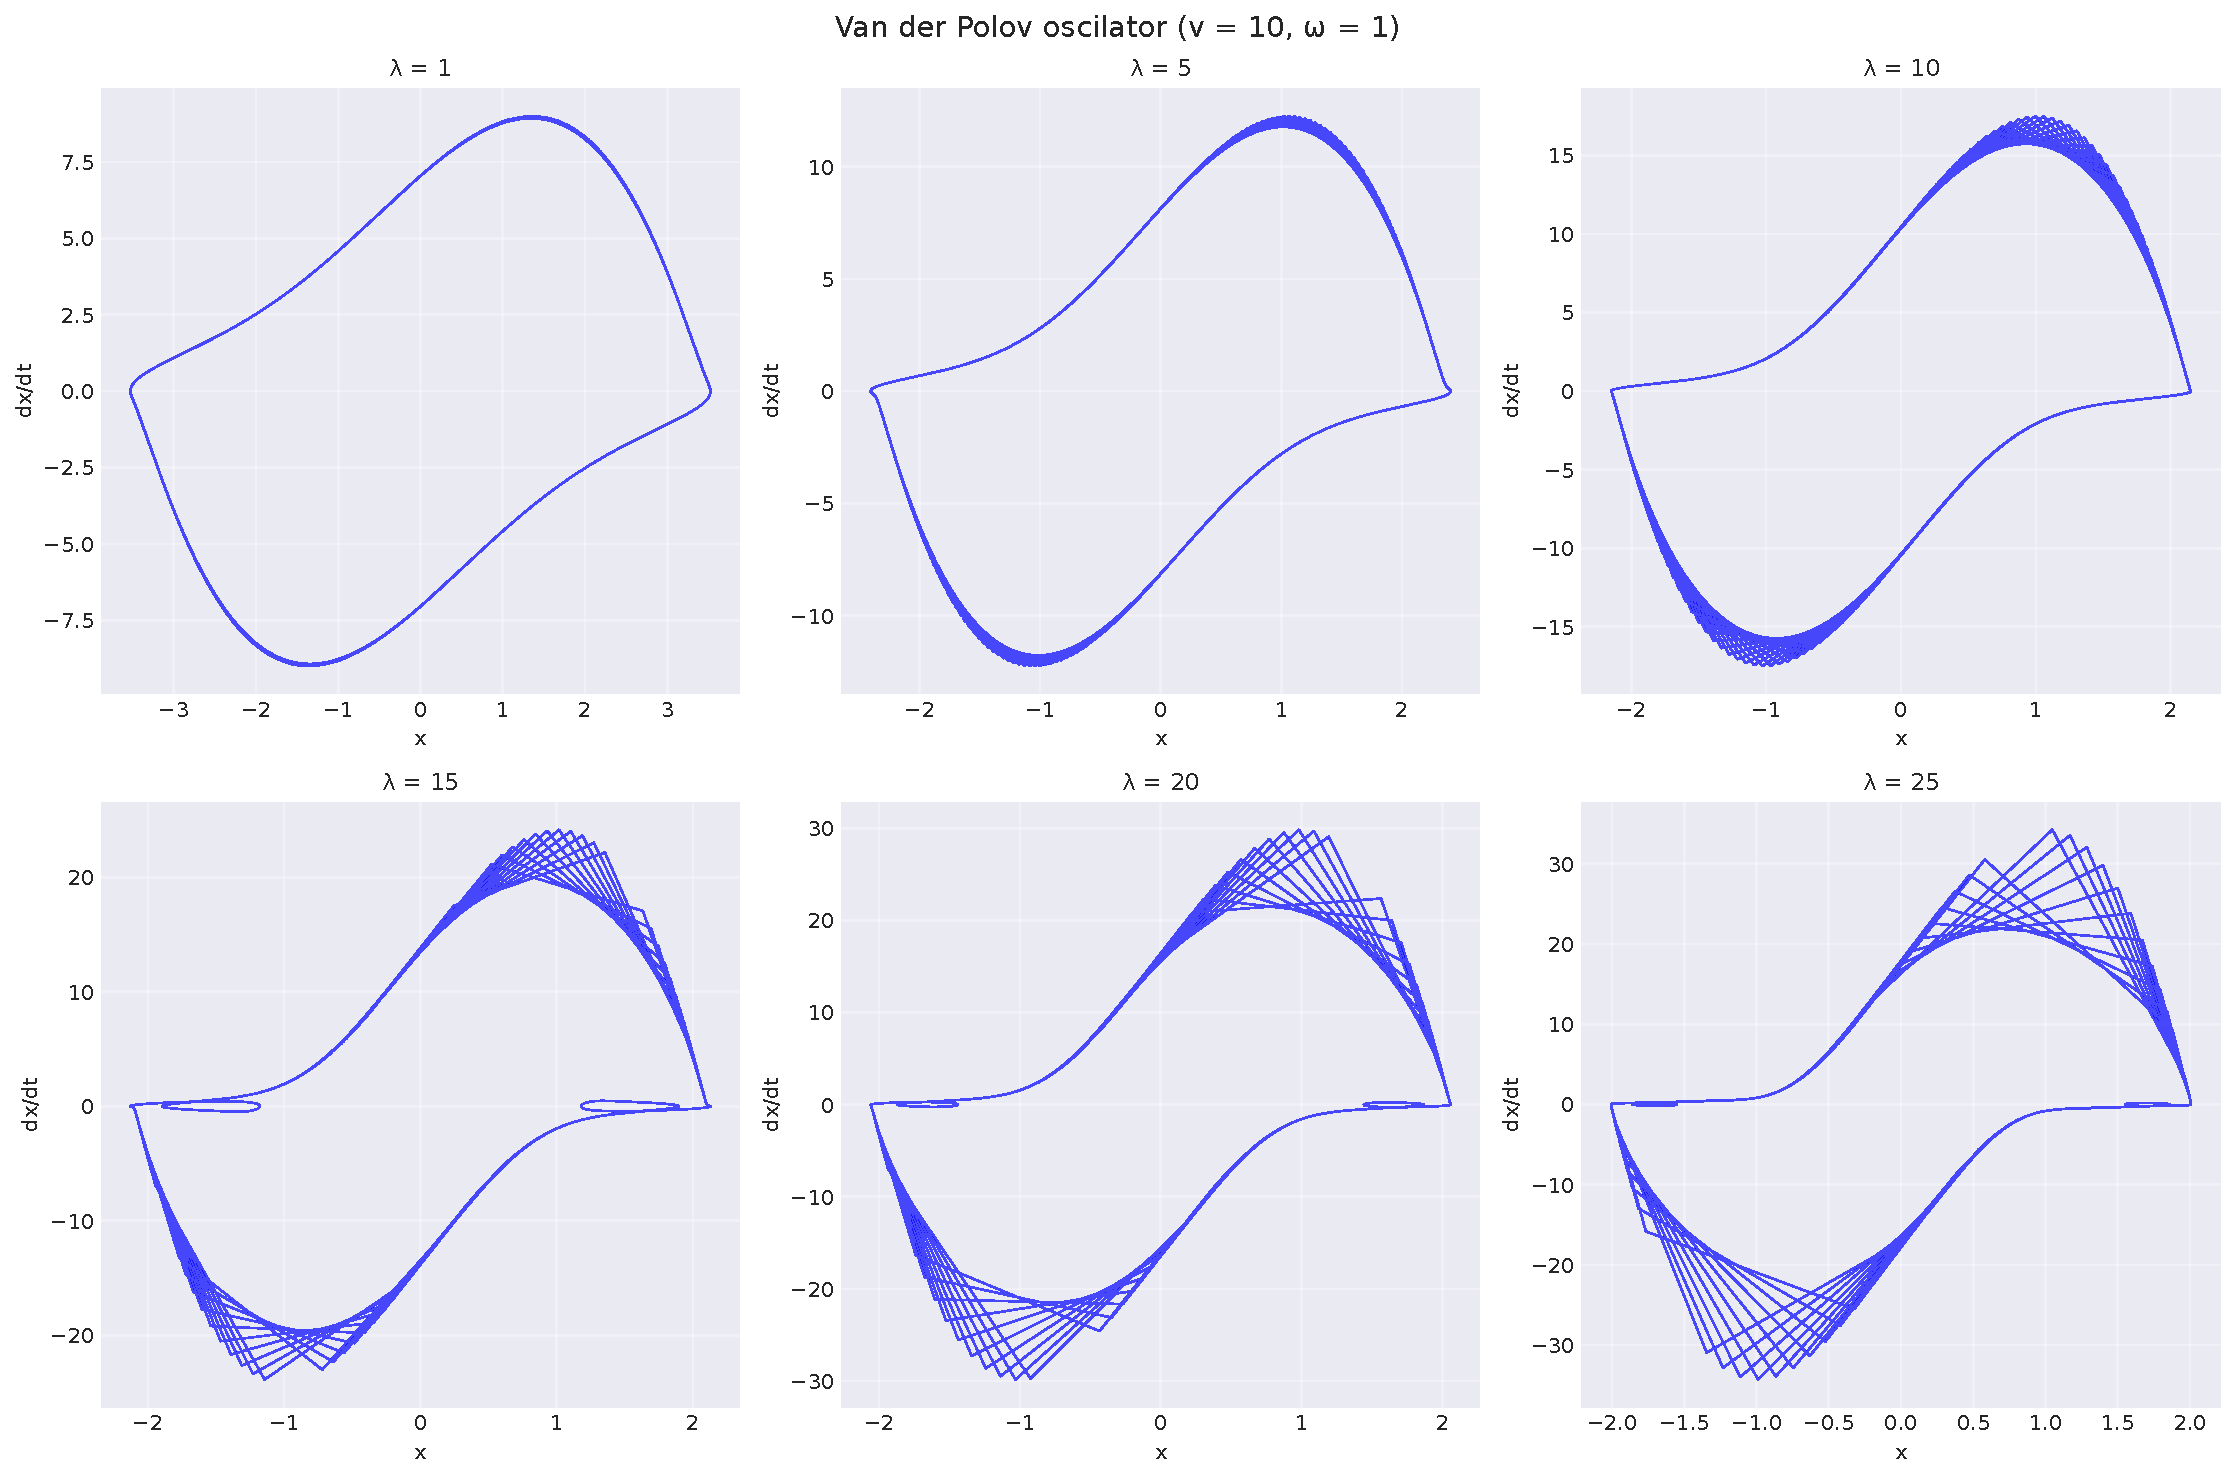
\includegraphics[width=0.9\textwidth]{slika14_vanderpol.pdf}
    \caption{Fazni portreti van der Polovega oscilatorja za različne vrednosti parametra $\lambda$ pri $v = 10$ in $\omega = 1$. Opazimo lahko prehod iz periodičnega nihanja v nihanje s trojno periodo pri $\lambda \approx 15$.}
    \label{fig:vanderpol}
\end{figure}

Pri majhnih vrednostih $\lambda$ (na primer $\lambda = 1$ in $\lambda = 5$) opazimo periodično nihanje, kjer je fazni portret skoraj krožnica, rahlo deformirana zaradi nelinearnosti. Ko $\lambda$ narašča, postaja limitni cikel vse bolj deformiran. Pri $\lambda = 10$ fazni portret še vedno kaže periodično nihanje, vendar je oblika že precej podolgovata. Pri $\lambda = 15$ opazimo pomembno spremembo: fazni portret kaže nihanje s trojno periodo, kar pomeni, da sistem potrebuje tri periode vzbujanja, da se vrne v isto stanje. To je primer bifurkacije s podvajanjem periode. Pri $\lambda = 20$ in $\lambda = 25$ postane nihanje še bolj kompleksno, z večjim številom vrtincev na faznem portretu.

\subsection{Hudičevo stopnišče}

Slika \ref{fig:devils_staircase} prikazuje zelo zanimiv pojav, znan kot hudičevo stopnišče. Graf prikazuje razmerje med lastno periodo oscilatorja in periodo vzbujanja v odvisnosti od parametra $\lambda$ za van der Polov oscilator pri $v = 1,2$ in $T_{\text{vzb}} = 10$ sekund.

\begin{figure}[H]
    \centering
    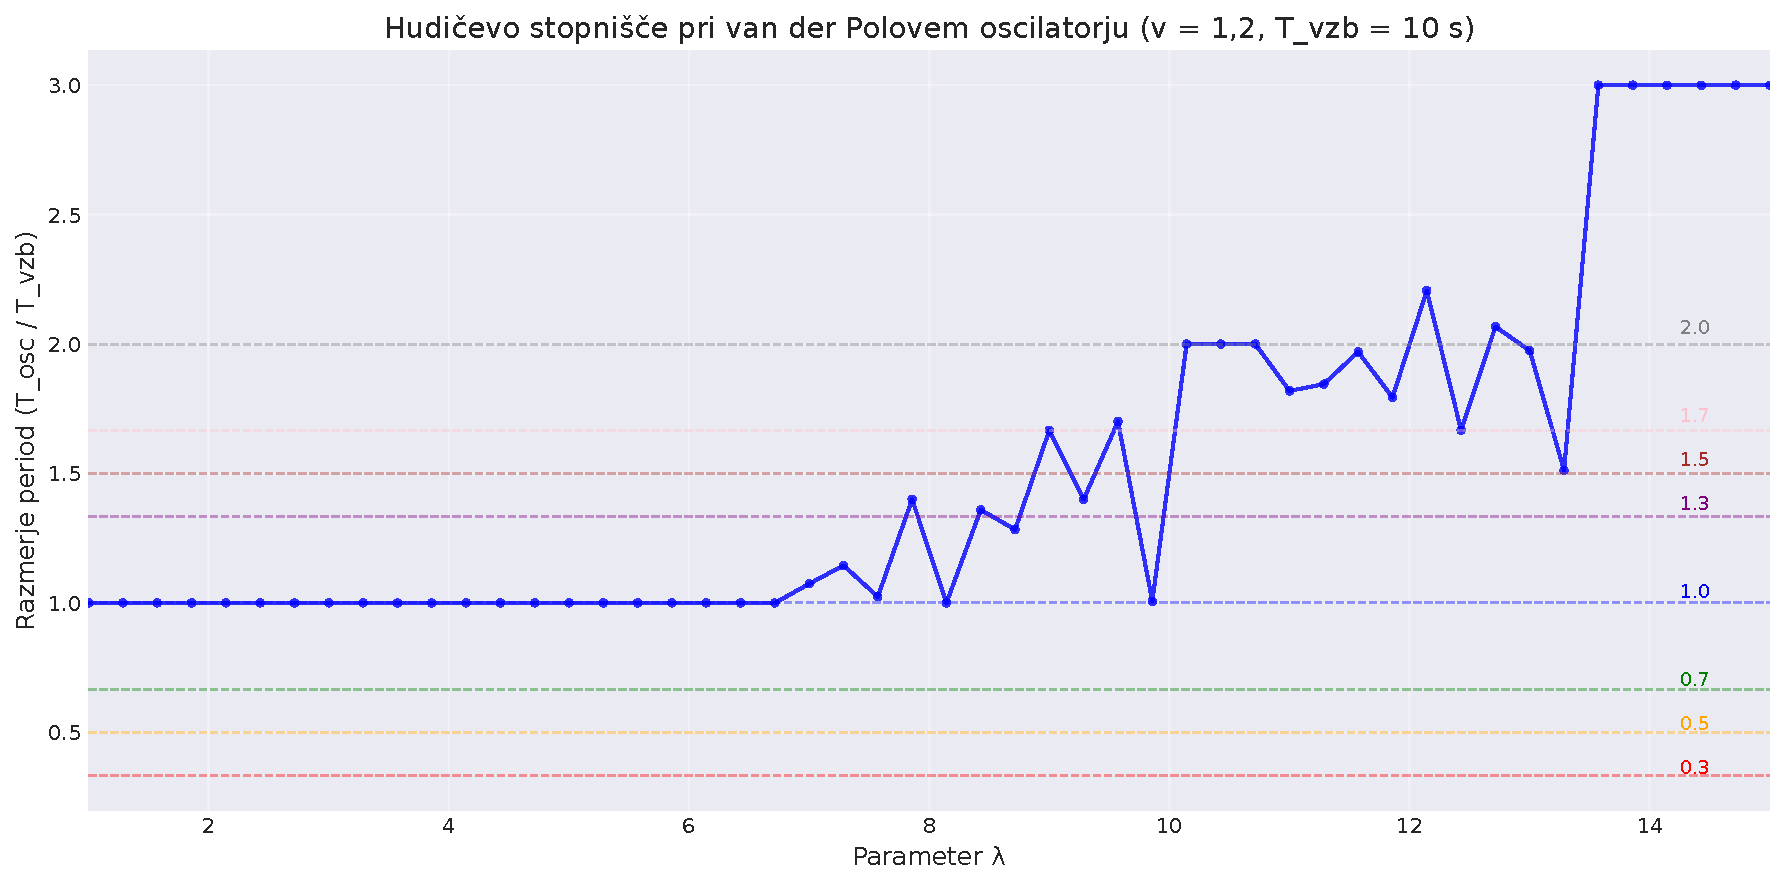
\includegraphics[width=0.9\textwidth]{slika16_hudicevo_stopnisce.pdf}
    \caption{Hudičevo stopnišče pri van der Polovem oscilatorju. Pri določenih vrednostih parametra $\lambda$ se lastna perioda oscilatorja ustali na racionalnih večkratnikih periode vzbujanja, kar tvori fraktalno strukturo. Z vodoravnimi črtami so označena racionalna razmerja.}
    \label{fig:devils_staircase}
\end{figure}

Opazimo lahko, da se pri določenih vrednostih $\lambda$ lastna perioda oscilatorja ustali na racionalnih večkratnikih periode vzbujanja, na primer pri razmerjih $1/2$, $2/3$, $1$, $4/3$ in tako naprej. Graf je sestavljen iz platojev (območij, kjer je razmerje konstantno) in strmih prehodov med njimi. Ta struktura je fraktalna, kar pomeni, da se podobni vzorci ponavljajo na različnih skalirah. Pojav se imenuje hudičevo stopnišče, ker graf spominja na stopnišče, pojav pa je povezan s teorijo faznih prehodov in fraktalov. Numerična simulacija tega pojava je zahtevna, saj zahteva zelo dolge simulacije (veliko tisoč period) in visoko natančnost, da se lahko zanesljivo določi, ali je razmerje period res racionalno ali le približno racionalno.

\section{Zaključek}

V okviru te naloge smo uspešno implementirali in primerjali pet različnih numeričnih metod za reševanje gibanja matematičnega nihala. Ugotovili smo, da je Eulerjeva metoda preveč netočna in nestabilna za resne simulacije, saj za dosego treh decimalnih mest natančnosti zahteva izjemno majhen korak $5,3 \cdot 10^{-4}$ s, poleg tega pa energija sistema pri tej metodi izjemno hitro narašča. Heunova in Verletova metoda (oba drugega reda) sta že uporabni za krajše simulacije, vendar se Verletova metoda izkaže za boljšo zaradi simplektičnosti, saj ohranja energijo in periodo tudi pri daljših simulacijah. RK4 metoda (četrti red) je izjemno natančna in primerna za kratke in srednje dolge simulacije, vendar tudi pri njej napaka energije počasi narašča s časom. PEFRL metoda (simplektična, četrti red) se je izkazala za najboljšo izbiro za dolgoročne simulacije, saj združuje visoko natančnost s simplektičnostjo, kar pomeni, da ohranja energijo in periodo tudi pri zelo dolgih simulacijah.

V drugem delu naloge smo raziskovali vsiljeno dušeno nihalo in van der Polov oscilator. Pri vsiljenem dušenem nihalu smo opazili različne dinamične režime, vključno s periodičnim nihanjem, bifurkacijami s podvajanjem periode, kaotičnim obnašanjem in navijanjem. Pri resonančnih krivuljah smo opazili pojav histereze, kjer ima sistem pri isti frekvenci vzbujanja lahko dva različna stabilna odziva. Pri van der Polovem oscilatorju pa smo opazili prehod iz periodičnega nihanja v nihanje s trojno periodo ter pojav hudičevega stopnišča, kjer se lastna perioda oscilatorja ustali na racionalnih večkratnikih periode vzbujanja.

Vsi ti rezultati poudarjajo pomen izbire ustrezne numerične metode glede na problem, ki ga rešujemo. Za kratkotrajne simulacije so metode višjega reda, kot sta RK4 in PEFRL, najprimernejše zaradi visoke natančnosti. Za dolgotrajne simulacije dinamičnih sistemov, kjer je pomembno ohranjanje energije in drugih invariant, pa so simplektične metode, zlasti Verletova in PEFRL, nepogrešljive. Razumevanje teh metod in njihovih lastnosti je ključno za uspešno numerično modeliranje fizikalnih pojavov.

\end{document}
